\documentclass[]{article}
\usepackage{lmodern}
\usepackage{setspace}
\setstretch{2}
\usepackage{amssymb,amsmath}
\usepackage{ifxetex,ifluatex}
\usepackage{fixltx2e} % provides \textsubscript
\ifnum 0\ifxetex 1\fi\ifluatex 1\fi=0 % if pdftex
  \usepackage[T1]{fontenc}
  \usepackage[utf8]{inputenc}
\else % if luatex or xelatex
  \ifxetex
    \usepackage{mathspec}
  \else
    \usepackage{fontspec}
  \fi
  \defaultfontfeatures{Ligatures=TeX,Scale=MatchLowercase}
\fi
% use upquote if available, for straight quotes in verbatim environments
\IfFileExists{upquote.sty}{\usepackage{upquote}}{}
% use microtype if available
\IfFileExists{microtype.sty}{%
\usepackage{microtype}
\UseMicrotypeSet[protrusion]{basicmath} % disable protrusion for tt fonts
}{}
\usepackage[margin = 1in]{geometry}
\usepackage{hyperref}
\hypersetup{unicode=true,
            pdfborder={0 0 0},
            breaklinks=true}
\urlstyle{same}  % don't use monospace font for urls
\usepackage{longtable,booktabs}
\usepackage{graphicx,grffile}
\makeatletter
\def\maxwidth{\ifdim\Gin@nat@width>\linewidth\linewidth\else\Gin@nat@width\fi}
\def\maxheight{\ifdim\Gin@nat@height>\textheight\textheight\else\Gin@nat@height\fi}
\makeatother
% Scale images if necessary, so that they will not overflow the page
% margins by default, and it is still possible to overwrite the defaults
% using explicit options in \includegraphics[width, height, ...]{}
\setkeys{Gin}{width=\maxwidth,height=\maxheight,keepaspectratio}
\IfFileExists{parskip.sty}{%
\usepackage{parskip}
}{% else
\setlength{\parindent}{0pt}
\setlength{\parskip}{6pt plus 2pt minus 1pt}
}
\setlength{\emergencystretch}{3em}  % prevent overfull lines
\providecommand{\tightlist}{%
  \setlength{\itemsep}{0pt}\setlength{\parskip}{0pt}}
\setcounter{secnumdepth}{5}
% Redefines (sub)paragraphs to behave more like sections
\ifx\paragraph\undefined\else
\let\oldparagraph\paragraph
\renewcommand{\paragraph}[1]{\oldparagraph{#1}\mbox{}}
\fi
\ifx\subparagraph\undefined\else
\let\oldsubparagraph\subparagraph
\renewcommand{\subparagraph}[1]{\oldsubparagraph{#1}\mbox{}}
\fi

%%% Use protect on footnotes to avoid problems with footnotes in titles
\let\rmarkdownfootnote\footnote%
\def\footnote{\protect\rmarkdownfootnote}

%%% Change title format to be more compact
\usepackage{titling}

% Create subtitle command for use in maketitle
\providecommand{\subtitle}[1]{
  \posttitle{
    \begin{center}\large#1\end{center}
    }
}

\setlength{\droptitle}{-2em}

  \title{}
    \pretitle{\vspace{\droptitle}}
  \posttitle{}
    \author{}
    \preauthor{}\postauthor{}
    \date{}
    \predate{}\postdate{}
  
\usepackage[left]{lineno}
\linenumbers

\begin{document}

Time of lineage divergence
constitutes a fundamental piece of information for evolutionary
understanding in many areas of research, from developmental to conservation biology ({\textbf{???}}; Webb \protect\hyperlink{ref-Webb2000}{2000}). This information can be obtained from fossils and from molecular dating studies. The developments in DNA sequencing and phylogenetic dating inferences have encouraged/spurred the application of molecular dating methods to a very large diversity of organisms, greatly increasing the quantity
of data on taxon ages across the tree of life.
Along with phylogenetic relationships, it allows testing alternative
evolutionary hypothesis in many areas of research, from developmental to conservation biology ({\textbf{???}}; Webb \protect\hyperlink{ref-Webb2000}{2000}).
It has been shown that only a bit of information on time of divergence can improve inferences of phylogenetic distance Webb et al. (\protect\hyperlink{ref-Webb2008}{2008}) bladj
Together with geographical distribution patterns, it is a crucial component of historical biogeography studies (Posadas et al. \protect\hyperlink{ref-posadas2006historical}{2006}).
Coupled to species number, it allows studying the tempo and mode of speciation and extinction,
central for understanding how biodiversity
patterns are shaped across space, time, and clades (Morlon \protect\hyperlink{ref-Morlon2014}{2014}).
In the past two decades, the possibility to obtain good quality DNA sequences
coupled to methodological developments in phylogenetic and dating inference, allowed
the application of molecular dating methods to a very large diversity
of organisms, greatly increasing the quantity and quality of data on taxon ages across the tree of life.
To date, there is a large amount of
data on taxon ages and phylogenetic relationships in public repositories such as Dryad, TreeBASE
and Open Tree of Life (OToL).
, --\textgreater{}

The TimeTree project (Hedges et al. \protect\hyperlink{ref-Hedges2006}{2006}, \protect\hyperlink{ref-Hedges2015}{2015}; Kumar et al. \protect\hyperlink{ref-Kumar2017}{2017}) has aggregated chronograms
from 3,163 studies, encompassing 97,085 species (Kumar et al. \protect\hyperlink{ref-Kumar2017}{2017}), and continues to grow.
However, even in this gold standard resource, the included taxa only encompass between
0.097 and 3.236\% of total species diversity (following taxonomic expert opinion
on the global, extant species numbers, which ranges from 3 to 100 million species
{[}Mayr2010; Moran2011{]}). One advantage of TimeTree is that it includes taxa from
across the tree of life, versus more specialized chronogram repositories focusing on land plants
(Stevens and Davis \protect\hyperlink{ref-stevens2001apw}{2001}) and mammals (Webb and Donoghue \protect\hyperlink{ref-webb2005phylomatic}{2005}), birds (Jetz et al. \protect\hyperlink{ref-Jetz2012}{2012}), and fish (Chang et al. \protect\hyperlink{ref-chang2019r}{2019}). Users can choose
between a web interface or a mobile app to receive information on divergence times
for the evolutionary history of a lineage, pairs of taxa, all lineages within a
taxon, or a list of taxa. As a science communication tool, TimeTree project is
very powerful: it has a friendly graphical interface, with informative and colorful
outputs, that allows the general public to satisfy curiosity regarding a particular
organism of interest or group of them. It is of limited utility for scientific
studies, however. The thousands of trees that have been entered are unavailable
for examination or reuse; according to the creators (see TimeTree web FAQ), methods
for allowing data downloading have been under discussion for the past several years
yet the primary data remain closed. Moreover, there is no Application Programming
Interface (API) allowing programmatic access to any data, greatly impairing the
possibility of large-scale, automated data-mining, which is not allowed under TimeTree
website's terms of use. The nearly hundred thousand taxon summary chronogram generated
from TimeTree resources is not available with its publication (Kumar et al. \protect\hyperlink{ref-Kumar2017}{2017}) or the
TimeTree website, though the still substantial chronogram from a previous publication
(Hedges et al. \protect\hyperlink{ref-Hedges2015}{2015}) was made available at OToL.

Despite its great importance, analytical tools to summarize available information
on taxon ages for the scientific community are still lacking.
We identified several aspects that might have so far delayed the exploitation of
existing data. First, original chronograms available publicly are scattered across repositories
and journals supplementary data, usually with different formats too.
Second, lineage names due to taxonomic idiosincracy can be different among studies
and manual curation of that is usually necessary.
Third, data curation

Platforms that contribute to knowledge in this areas:

Supersmart is an open tool but not easy to use, still requires a lot of curation and knowledge.

Phylogenerator ({\textbf{???}})

Generate new dates using all available DNA sequence information;
Perform one global analysis using all available information;

Problems or downsides: This might be time consuming for large groups and a lot of
data curation and knowledge on the group of interest is still necessary. For example,
choosing correct fossils for calibration
requires a lot of expertise and knowledge on the group. An incorrect use of fossils
can generate severe bias in dating results (Sauquet et al. \protect\hyperlink{ref-Sauquet2012c}{2012}).
Hence, data curation is still an important part of any biological study. The research
community considers it as an important or even crucial step before data analysis.
Hence, automated processes for large data analysis are frequently received with skepticism.

\texttt{datelife} palliates this by only using information available from already published
studies, which are ideally constructed using robust information, such as sequence
data and thoughtfully curated fossil calibrations.

Rapidly increasing data on time of lineage divergence both from molecular and paleontological studies; the increasing importance of use of these data in distant areas of research, often not specialized enough to rapidly obain data on their own; and the lack of an open (both the data sources and the code underlying the analyses) easy to use tool
inspired the development of a prototype \texttt{datelife} service over a series
of phylotastic hackathons (Stoltzfus et al. \protect\hyperlink{ref-Stoltzfus2013}{2013}) at the National Evolutionary Synthesis Center.
In this paper we present the first formal description of \texttt{datelife}, featuring an improved database of chronograms, more methods to summarize trees, and new functions to visualize data, as well as comparisons of summary trees.
\texttt{datelife} is the main service for scaling phylogenetic trees in Phylotastic! system
(Stoltzfus et al. \protect\hyperlink{ref-Stoltzfus2013}{2013})
It can be used through its R package , and a web interface
(\url{http://www.datelife.org/query/}).

\hypertarget{refs}{}
\leavevmode\hypertarget{ref-barker2012going}{}%
Barker F.K., Burns K.J., Klicka J., Lanyon S.M., Lovette I.J. 2012. Going to extremes: Contrasting rates of diversification in a recent radiation of new world passerine birds. Systematic biology. 62:298--320.

\leavevmode\hypertarget{ref-barker2015new}{}%
Barker F.K., Burns K.J., Klicka J., Lanyon S.M., Lovette I.J. 2015. New insights into new world biogeography: An integrated view from the phylogeny of blackbirds, cardinals, sparrows, tanagers, warblers, and allies. The Auk: Ornithological Advances. 132:333--348.

\leavevmode\hypertarget{ref-burns2014phylogenetics}{}%
Burns K.J., Shultz A.J., Title P.O., Mason N.A., Barker F.K., Klicka J., Lanyon S.M., Lovette I.J. 2014. Phylogenetics and diversification of tanagers (passeriformes: Thraupidae), the largest radiation of neotropical songbirds. Molecular Phylogenetics and Evolution. 75:41--77.

\leavevmode\hypertarget{ref-chang2019r}{}%
Chang J., Rabosky D.L., Smith S.A., Alfaro M.E. 2019. An r package and online resource for macroevolutionary studies using the ray-finned fish tree of life. Methods in Ecology and Evolution. 0:1--7.

\leavevmode\hypertarget{ref-claramunt2015new}{}%
Claramunt S., Cracraft J. 2015. A new time tree reveals earth history's imprint on the evolution of modern birds. Science advances. 1:e1501005.

\leavevmode\hypertarget{ref-gibb2015new}{}%
Gibb G.C., England R., Hartig G., McLenachan P.A., Taylor Smith B.L., McComish B.J., Cooper A., Penny D. 2015. New zealand passerines help clarify the diversification of major songbird lineages during the oligocene. Genome biology and evolution. 7:2983--2995.

\leavevmode\hypertarget{ref-Hedges2006}{}%
Hedges S.B., Dudley J., Kumar S. 2006. TimeTree: A public knowledge-base of divergence times among organisms. Bioinformatics. 22:2971--2972.

\leavevmode\hypertarget{ref-Hedges2015}{}%
Hedges S.B., Marin J., Suleski M., Paymer M., Kumar S. 2015. Tree of life reveals clock-like speciation and diversification. Molecular Biology and Evolution. 32:835--845.

\leavevmode\hypertarget{ref-hooper2017chromosomal}{}%
Hooper D.M., Price T.D. 2017. Chromosomal inversion differences correlate with range overlap in passerine birds. Nature ecology \& evolution. 1:1526.

\leavevmode\hypertarget{ref-Jetz2012}{}%
Jetz W., Thomas G., Joy J.J., Hartmann K., Mooers A. 2012. The global diversity of birds in space and time. Nature. 491:444--448.

\leavevmode\hypertarget{ref-Kumar2017}{}%
Kumar S., Stecher G., Suleski M., Hedges S.B. 2017. TimeTree: A Resource for Timelines, Timetrees, and Divergence Times. Molecular biology and evolution. 34:1812--1819.

\leavevmode\hypertarget{ref-Morlon2014}{}%
Morlon H. 2014. Phylogenetic approaches for studying diversification. Ecology Letters. 17:508--525.

\leavevmode\hypertarget{ref-posadas2006historical}{}%
Posadas P., Crisci J.V., Katinas L. 2006. Historical biogeography: A review of its basic concepts and critical issues. Journal of Arid Environments. 66:389--403.

\leavevmode\hypertarget{ref-price2014niche}{}%
Price T.D., Hooper D.M., Buchanan C.D., Johansson U.S., Tietze D.T., Alström P., Olsson U., Ghosh-Harihar M., Ishtiaq F., Gupta S.K., others. 2014. Niche filling slows the diversification of himalayan songbirds. Nature. 509:222.

\leavevmode\hypertarget{ref-Sauquet2012c}{}%
Sauquet H., Ho S.Y.W., Gandolfo M. a, Jordan G.J., Wilf P., Cantrill D.J., Bayly M.J., Bromham L., Brown G.K., Carpenter R.J., Lee D.M., Murphy D.J., Sniderman J.M.K., Udovicic F. 2012. Testing the impact of calibration on molecular divergence times using a fossil-rich group: the case of Nothofagus (Fagales). Systematic Biology. 61:289--313.

\leavevmode\hypertarget{ref-stevens2001apw}{}%
Stevens P.F., Davis H. 2001. Angiosperm phylogeny website..

\leavevmode\hypertarget{ref-Stoltzfus2013}{}%
Stoltzfus A., Lapp H., Matasci N., Deus H., Sidlauskas B., Zmasek C.M., Vaidya G., Pontelli E., Cranston K., Vos R., Webb C.O., Harmon L.J., Pirrung M., O'Meara B., Pennell M.W., Mirarab S., Rosenberg M.S., Balhoff J.P., Bik H.M., Heath T.A., Midford P.E., Brown J.W., McTavish E.J., Sukumaran J., Westneat M., Alfaro M.E., Steele A., Jordan G. 2013. Phylotastic! Making tree-of-life knowledge accessible, reusable and convenient. BMC Bioinformatics. 14.

\leavevmode\hypertarget{ref-Webb2000}{}%
Webb C.O. 2000. Exploring the Phylogenetic Structure of Ecological Communities : An Example for Rain Forest Trees. The American Naturalist. 156:145--155.

\leavevmode\hypertarget{ref-Webb2008}{}%
Webb C.O., Ackerly D.D., Kembel S.W. 2008. Phylocom: Software for the analysis of phylogenetic community structure and trait evolution. Bioinformatics. 24:2098--2100.

\leavevmode\hypertarget{ref-webb2005phylomatic}{}%
Webb C.O., Donoghue M.J. 2005. Phylomatic: Tree assembly for applied phylogenetics. Molecular Ecology Notes. 5:181--183.

\newpage

\begin{center}
\textsc{Figure \ref{fig:workflow}}
\end{center}
Stylized DateLife workflow. This shows the general worflows and analyses that can be performed with \texttt{datelife}, via the R package or through the website. Details on the functions involved on each workflow are shown in \texttt{datelife}'s R package vignette.

\begin{center}
\textsc{Figure \ref{fig:runtime1}}
\end{center}
Computation time of query processing and search across \texttt{datelife}'s chronogram database relative to number of input taxon names. We sampled N names from the class Aves for each cohort 100 times and then performed a search with query processing not using the Taxon Names Resoultion Service (TNRS; dark gray), and using TNRS (light gray). We also performed a search using the already processed query for comparison (light blue). 

\begin{center}
\textsc{Figure \ref{fig:schronograms1}}
\end{center}
Lineage through time (LTT) plots of source chronograms containing all or a subset of species from the bird family Fringillidae of true finches. Arrows indicate maximum age of each chronogram. Numbers reference to chronograms' original publications 1: Barker et al. (\protect\hyperlink{ref-barker2012going}{2012}), 2: Barker et al. (\protect\hyperlink{ref-barker2015new}{2015}), 3: Burns et al. (\protect\hyperlink{ref-burns2014phylogenetics}{2014}), 4: Claramunt and Cracraft (\protect\hyperlink{ref-claramunt2015new}{2015}), 5: Gibb et al. (\protect\hyperlink{ref-gibb2015new}{2015}), 6: Hedges et al. (\protect\hyperlink{ref-Hedges2015}{2015}), 7: Hooper and Price (\protect\hyperlink{ref-hooper2017chromosomal}{2017}), 8: Jetz et al. (\protect\hyperlink{ref-Jetz2012}{2012}), 9: Price et al. (\protect\hyperlink{ref-price2014niche}{2014}).

\begin{center}
\textsc{Figure \ref{fig:summaries}}
\end{center}
LTT plots of median and Supermatrix Distance Method (SDM) chronograms summarising information from source chronograms found for the Fringillidae. Arrows indicate maximum age.

\begin{center}
\textsc{Figure \ref{fig:cvbladj}}
\end{center}
LTT plots showing results from the cross-validation analyses of trees without branch lengths dated using BLADJ. The dating analysis can only be performed in trees with more than 2 tips, thus excluding chronogram from study 4; its data was still used as calibration for the other source chronograms.

\begin{center}
\textsc{Figure \ref{fig:cvbold}}
\end{center}
LTT plots showing results from the cross-validation analyses of trees with branch length reconstructed with data from the Barcode of Life Database (BOLD) dated using PATHd8. We could construct a tree with branch lengths for all source chronograms. However, dating with PATHd8 was only successful in three source chronograms shown here.

\newpage

\begin{figure}[!h]
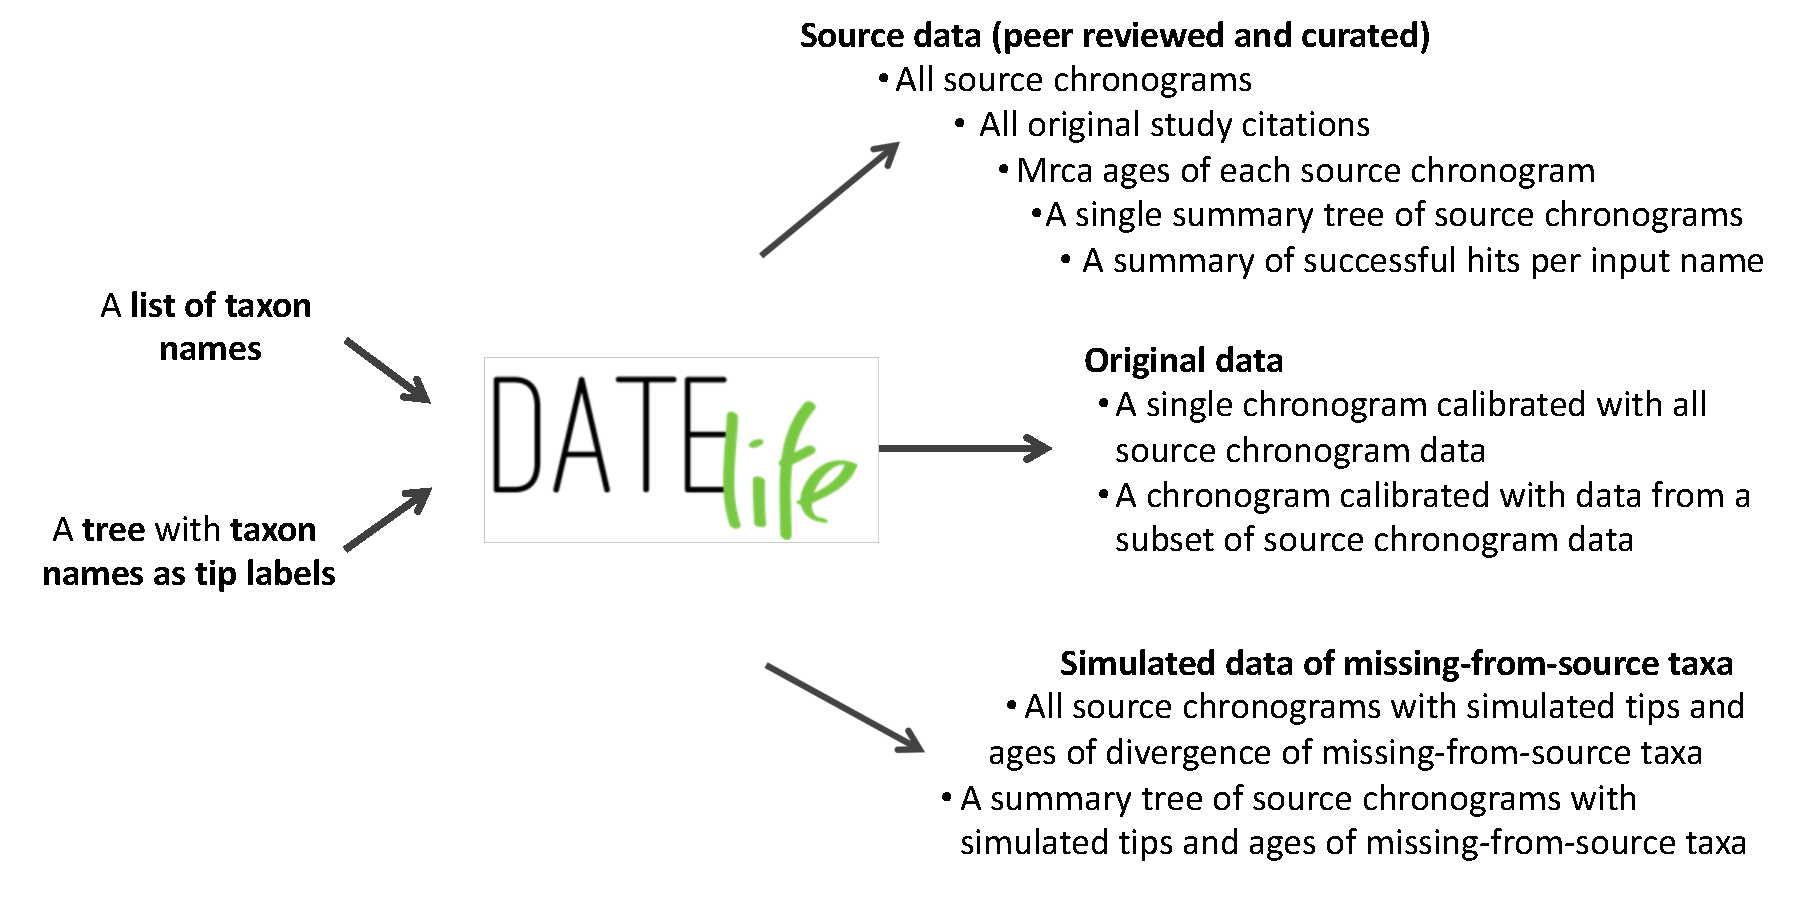
\includegraphics{Fig1.pdf}
\caption{}
\label{fig:workflow}
\end{figure}

\newpage

\begin{figure}[!h]
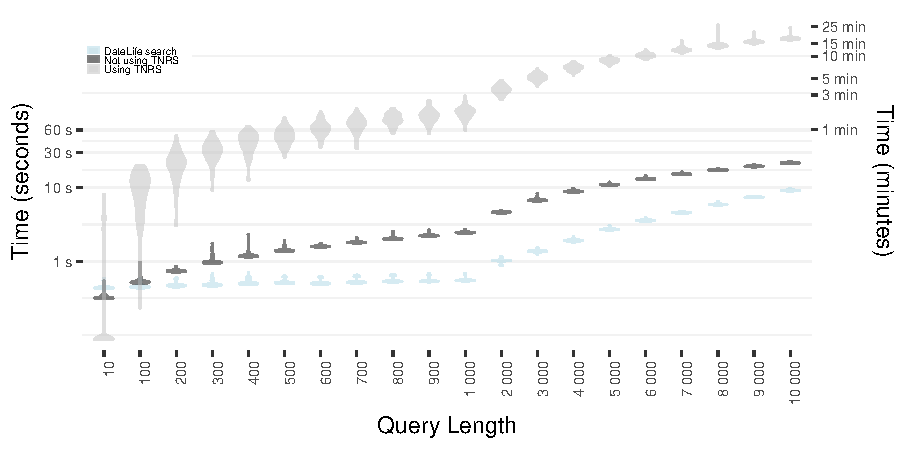
\includegraphics[width=1\linewidth]{fig_runtime1.pdf}
\caption{}
\label{fig:runtime1}
\end{figure}

\newpage

\begin{figure}[!h]
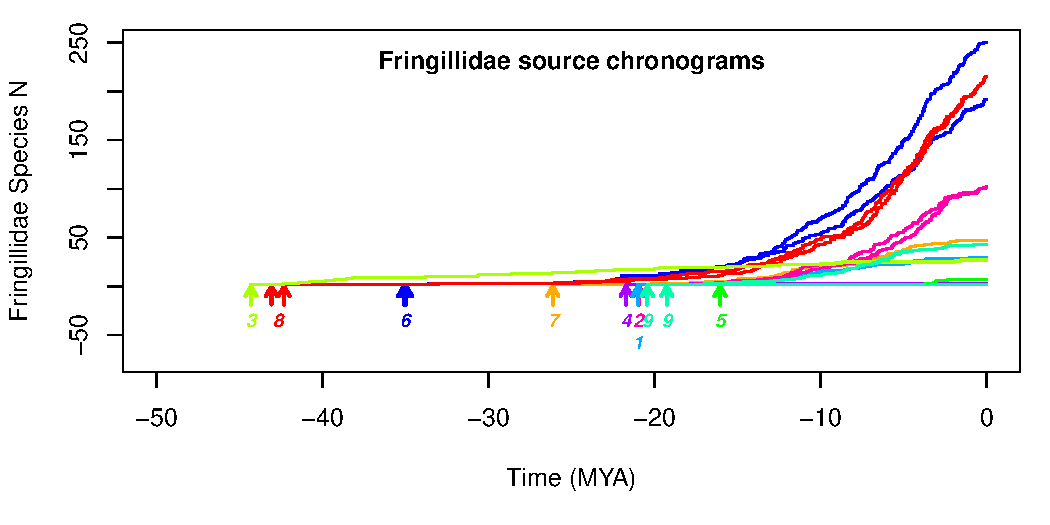
\includegraphics[width=1\linewidth]{fig_schronograms1.pdf}
\caption{}
\label{fig:schronograms1}
\end{figure}

\newpage

\begin{figure}[!h]
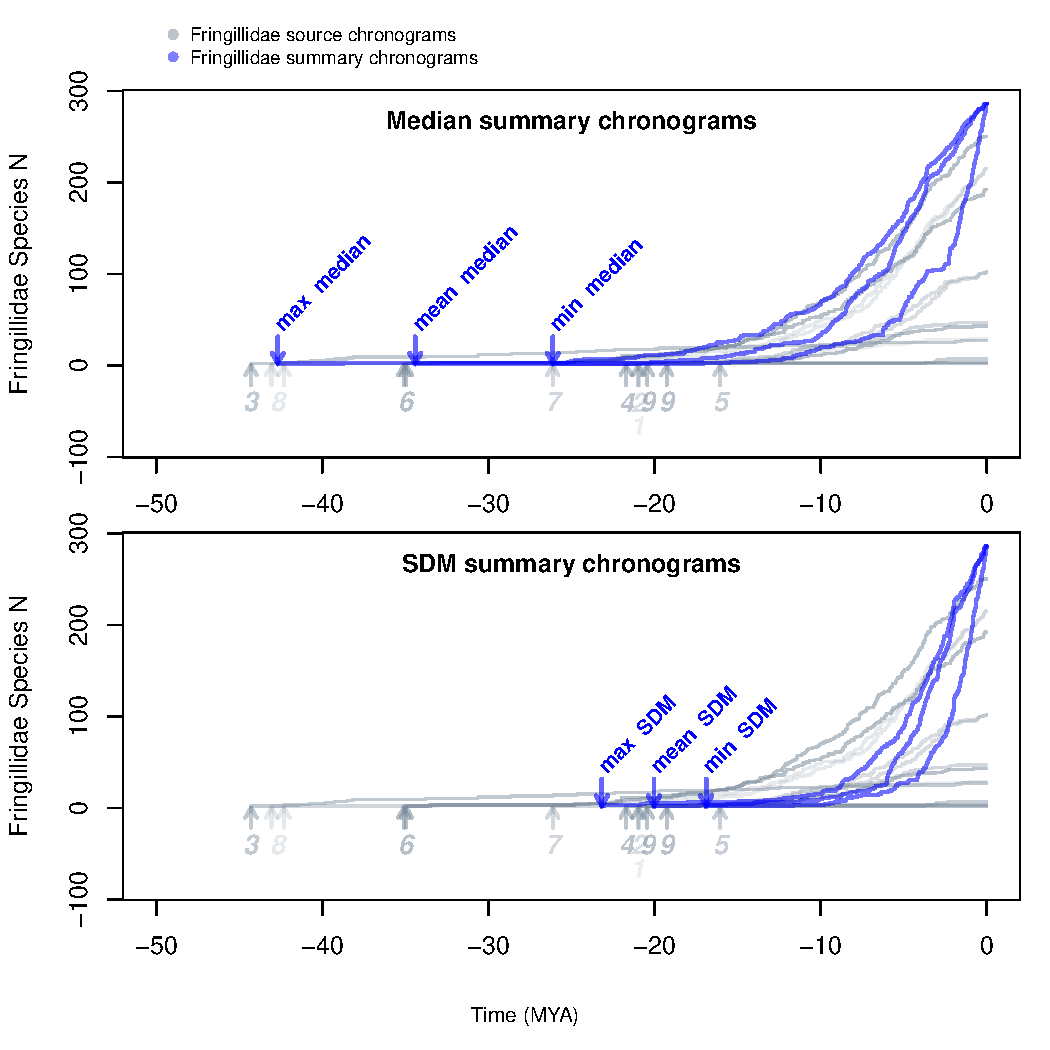
\includegraphics{fig_summaries.pdf}
%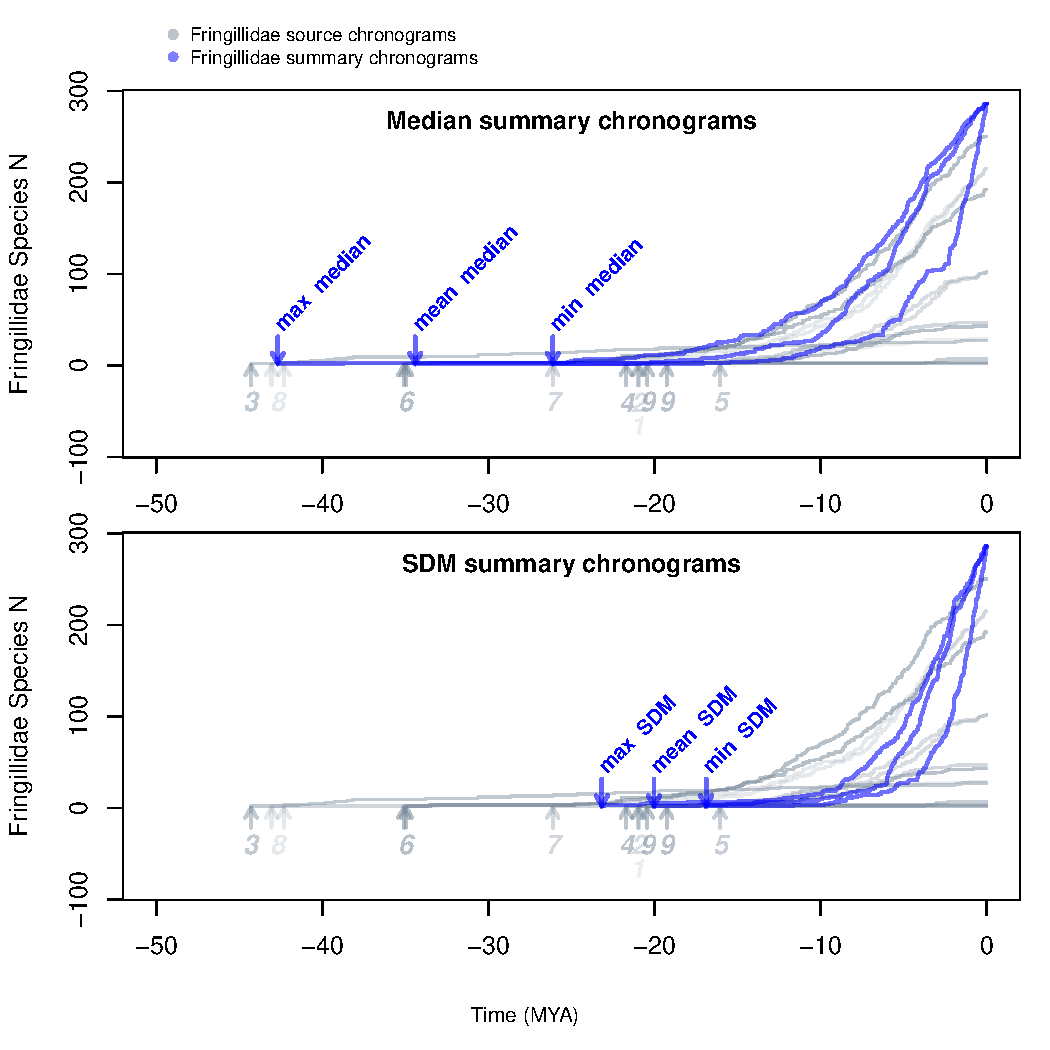
\includegraphics{fig_summaries.pdf}
\caption{}
\label{fig:summaries}
\end{figure}

\newpage

\begin{figure}[!h]
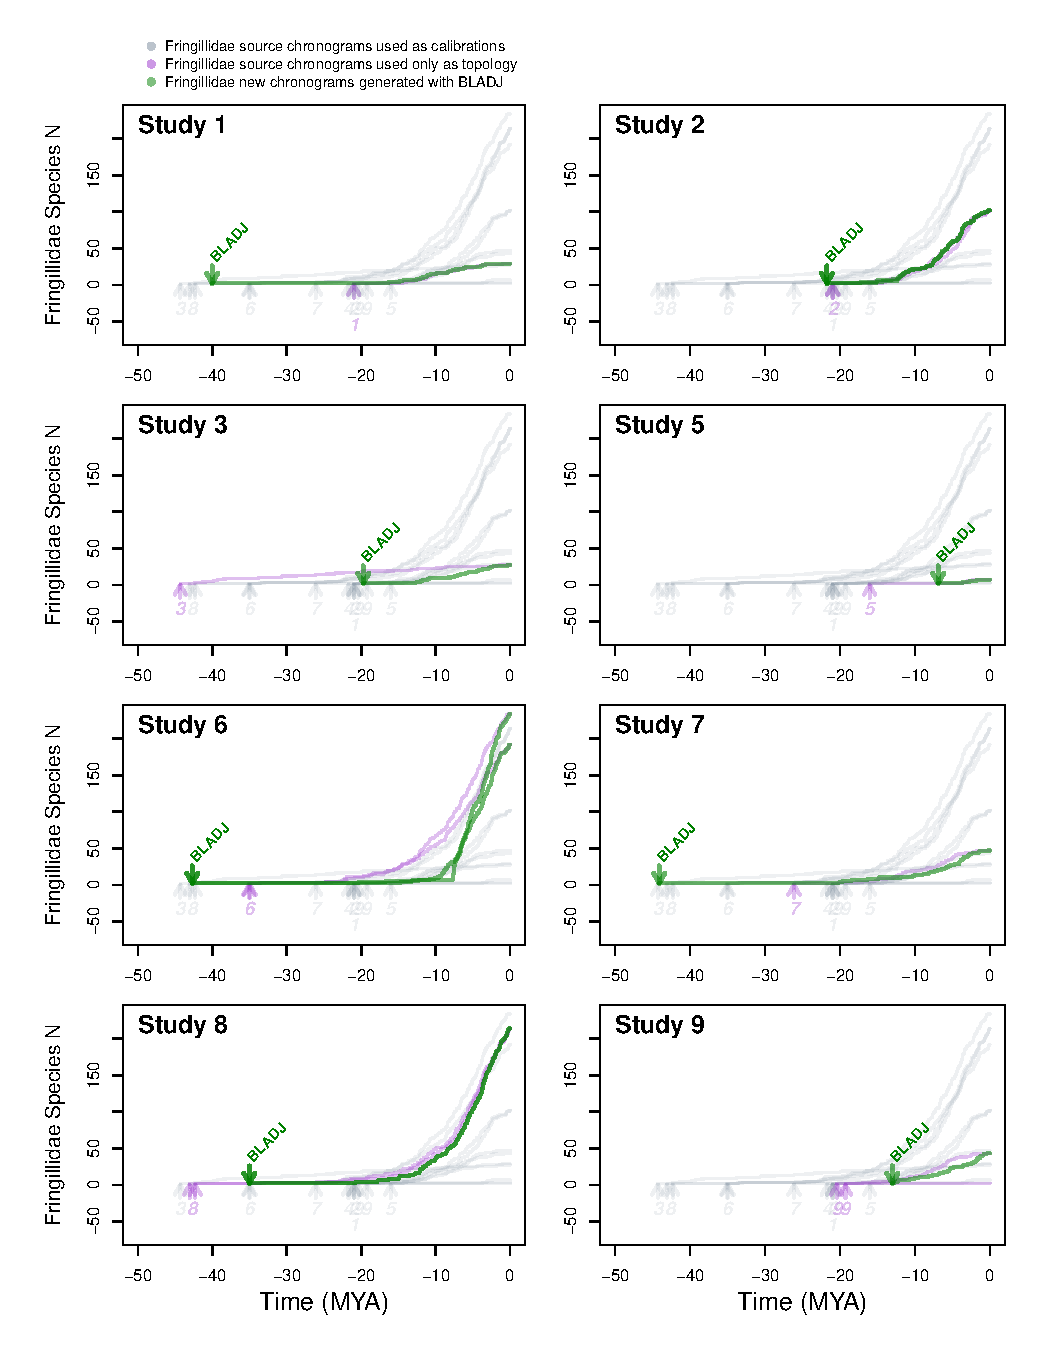
\includegraphics{fig_crossval_bladj.pdf}
\caption{}
\label{fig:cvbladj}
\end{figure}

\newpage

\begin{figure}[!h]
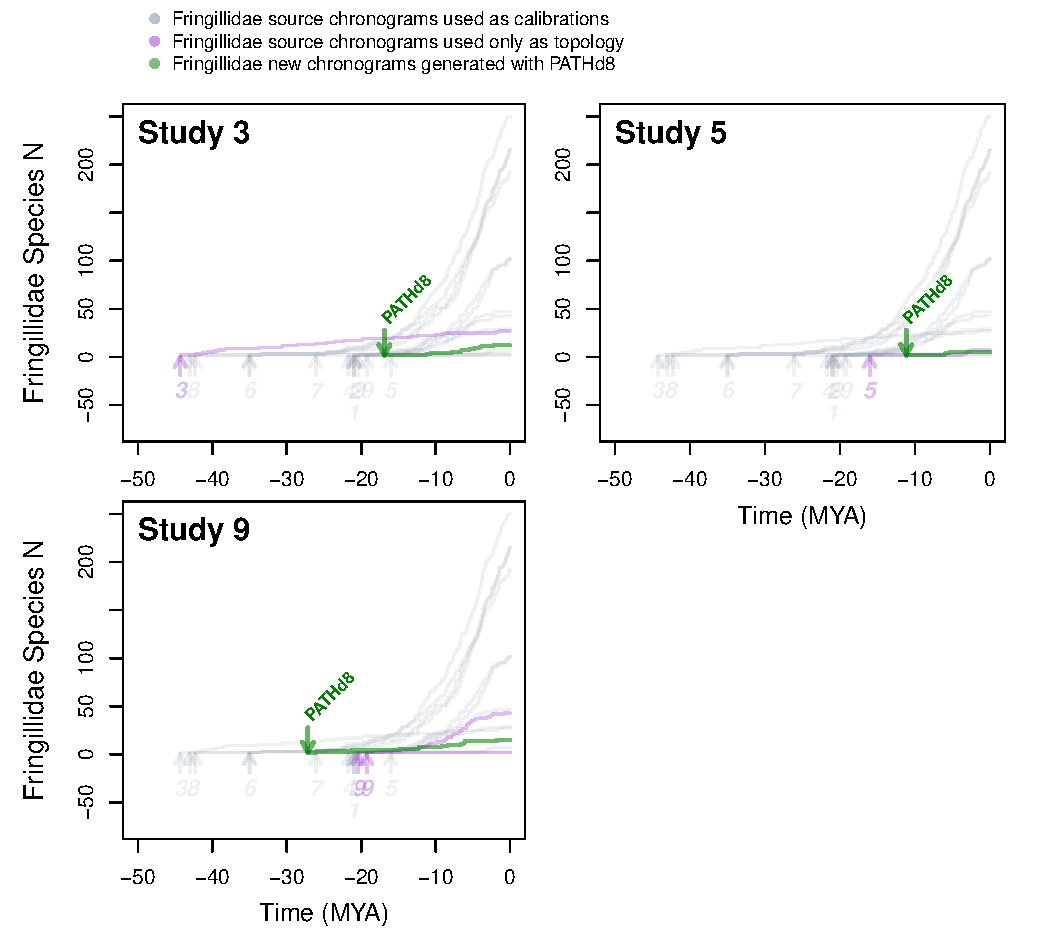
\includegraphics{fig_crossval_boldsumm.pdf}
\caption{}
\label{fig:cvbold}
\end{figure}


\end{document}
